%****************************************************************%
% FILE: funzionalita.tex                                        %
%****************************************************************%
\documentclass[./main.tex]{subfiles}

\begin{document}

L'applicazione dovrà fornire una serie di funzionalità, sia per quanto riguarda l'utilizzo vero e proprio dell'applicazione da parte dell'utente finale (\textit{front-end}), che per la parte sottostante dell'applicazione (\textit{back-end}). Inizialmente il cliente richiede un certo numero di funzionalità che desidera vedere implementate, nelle sezioni successive saranno infatti descritte. È chiaro che, dato il tempo limitato e la necessità di produrre qualcosa di concreto, le prime versioni del software avranno solamente le funzionalità ritenute prioritarie. Questa scala di priorità si affina quando, procedendo nello sviluppo, si giunge alla conclusione di uno sprint.\par

%\paragraph{Front-end.}%
Il \textbf{front-end} è la parte grafica dell'applicazione che l'utente utilizzerà dal suo dispositivo. Nonostante l'implementazione sia affidata ad un team esterno, risulta necessario approfondirla in quanto gli sviluppatori del back-end devono sapere quali dati e risorse dare al front-end per un corretto funzionamento del prodotto. In particolare, non essendo ancora stata avviata la produzione del front-end, si farà uso di un \textit{mockup} grafico, basato sulla precedente applicazione\footcite[https://www.ismar.cnr.it/terza-missione/app/\#2]{website-ismar-cnr}. Esso viene creato appositamente per dare un'idea di come dovrebbe presentarsi l'applicazione quando sarà terminata in modo da aiutare gli sviluppatori ad avere un obiettivo chiaro. In aggiunta, per presentare al cliente i vari progressi, viene sviluppata una \textit{demo web}\footnote{\textbf{demo} <démë> s. ingl. [abbrev. di demonstration «dimostrazione»] (pl. demos <démë$\int$>), usato in ital. al masch. o al femm. (e comunem. pronunciato <démo>). – In informatica, versione dimostrativa di un programma, presentato per lo più, a scopo di campagna pubblicitaria, in forma semplificata e parziale; \cite{treccani-demo}.}. Essa sarà usata, come valida alternativa all'applicazione vera e propria, nei successivi capitoli quando si analizzerà il lavoro fatto.\par

%\paragraph{Funzionalità e mockup grafico.}
L'applicazione, come illustrato in \autoref{fig:app_staz_oss_fisse}, visualizza una mappa, navigabile, nella quale compaiono alcuni cerchi numerati ad indicare la posizione delle stazioni osservative fisse. A questo si aggiunge, nella stessa schermata, la possibilità di visualizzare le stazioni sotto forma di elenco. Ogni località, se cliccata, visualizza una nuova finestra contenente i suoi dati meteorologici sotto forma di \textit{widget}\footnote{Con il termine \textit{widget} si intendono dei riquadri grafici, con cui l'utente può interagire, contenenti dati e altre informazioni.} e grafici, sulla base di cosa sarà necessario visualizzare. Ad esempio nella terza e quarta immagine si possono osservare alcuni widget relativi alla \textit{Piattaforma Acqua Alta} che indicano, in ordine, la velocità e direzione del vento, il tempo climatico (in questo caso nuvoloso), la temperatura atmosferica in un intervallo di tempo prefissato. Inoltre l'utente ha la possibilità di selezionare, tramite appositi riquadri, i dati della stazione che vuole visualizzare.

\begin{figure}[!ht]
\noindent\begin{minipage}{\textwidth}
\vspace{1cm}
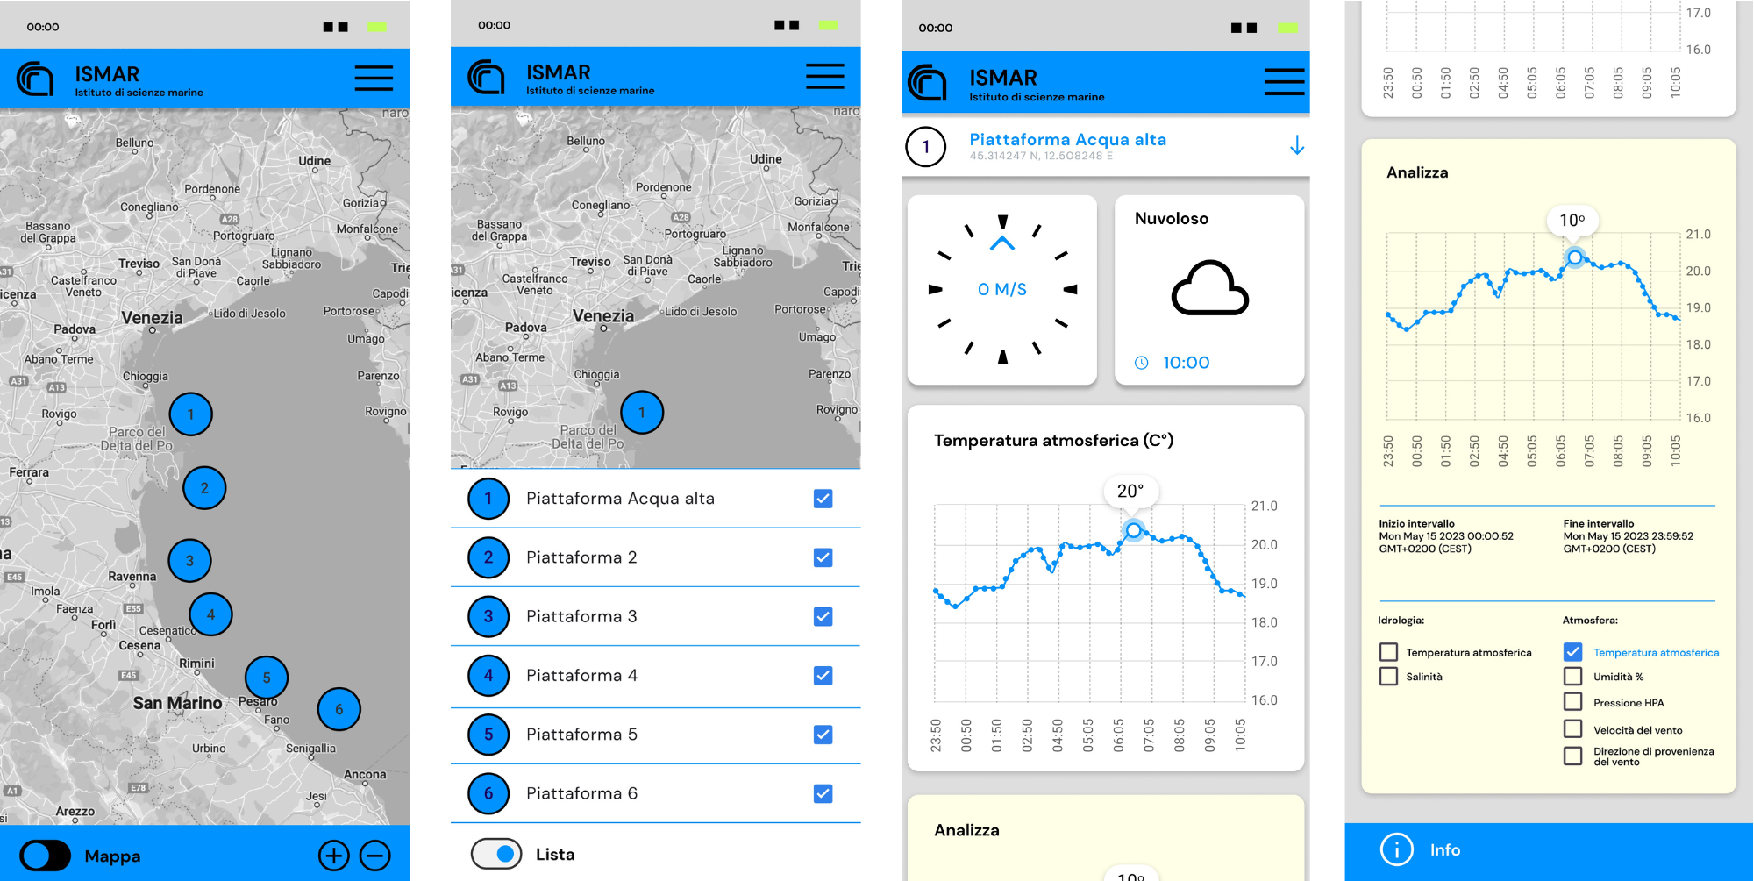
\includegraphics[width=\textwidth]{images/app_ismar_data_staz_oss_fisse.pdf}
\captionsetup{font=small, hypcap=false}
\captionof{figure}{Schermate stazioni osservative fisse: mappa, lista e \textit{widget}.\protect\footnote{Fonte: mockup grafico.}.}
\label{fig:app_staz_oss_fisse}
\end{minipage}
\vspace{0.25cm}
\end{figure}

È presente un menu, in \autoref{fig:app_menu_henetus}, contenente le seguenti opzioni che si occupano di visualizzare schermate differenti a seconda della preferenza scelta:
\begin{itemize}
    \item \textit{Mappa}: mappa delle stazioni osservative fisse.
    \item \textit{Modelli di previsione}: mappe con le previsioni di onde e venti prodotte dai sistemi Nettuno ed Henetus.
    \item \textit{Osservazioni da satellite}: mappe contenenti i dati di clorofilla e temperatura superficiale del mare rilevate dai satelliti.
    \item \textit{Radar}: mappa contenete i dati rilevati dai radar.
    \item \textit{Info}: informazioni generali sull'applicazione.
    \item \textit{Webcam}: immagini prese dalle webcam poste sulle stazioni osservative fisse.
\end{itemize}

L'esempio continua mostrando, nelle schermate successive al menu, la mappa con le freccette e i colori ad indicare rispettivamente direzione del vento e altezza d'onda rilevate dal modello di previsione Nettuno. Anche qua tramite appositi riquadri è possibile selezionare alcuni filtri, come l'area geografica di interesse. Infine è presente una breve descrizione del sistema visualizzato per spiegare di cosa si occupa Nettuno.

Le informazioni dettagliate su quali dati visualizzare per ogni sorgente saranno discusse nel corso del documento. Al momento, per le finalità del presente paragrafo, non risulta necessario affrontare quell'argomento.

\begin{figure}[!ht]
\noindent\begin{minipage}{\textwidth}
\vspace{1cm}
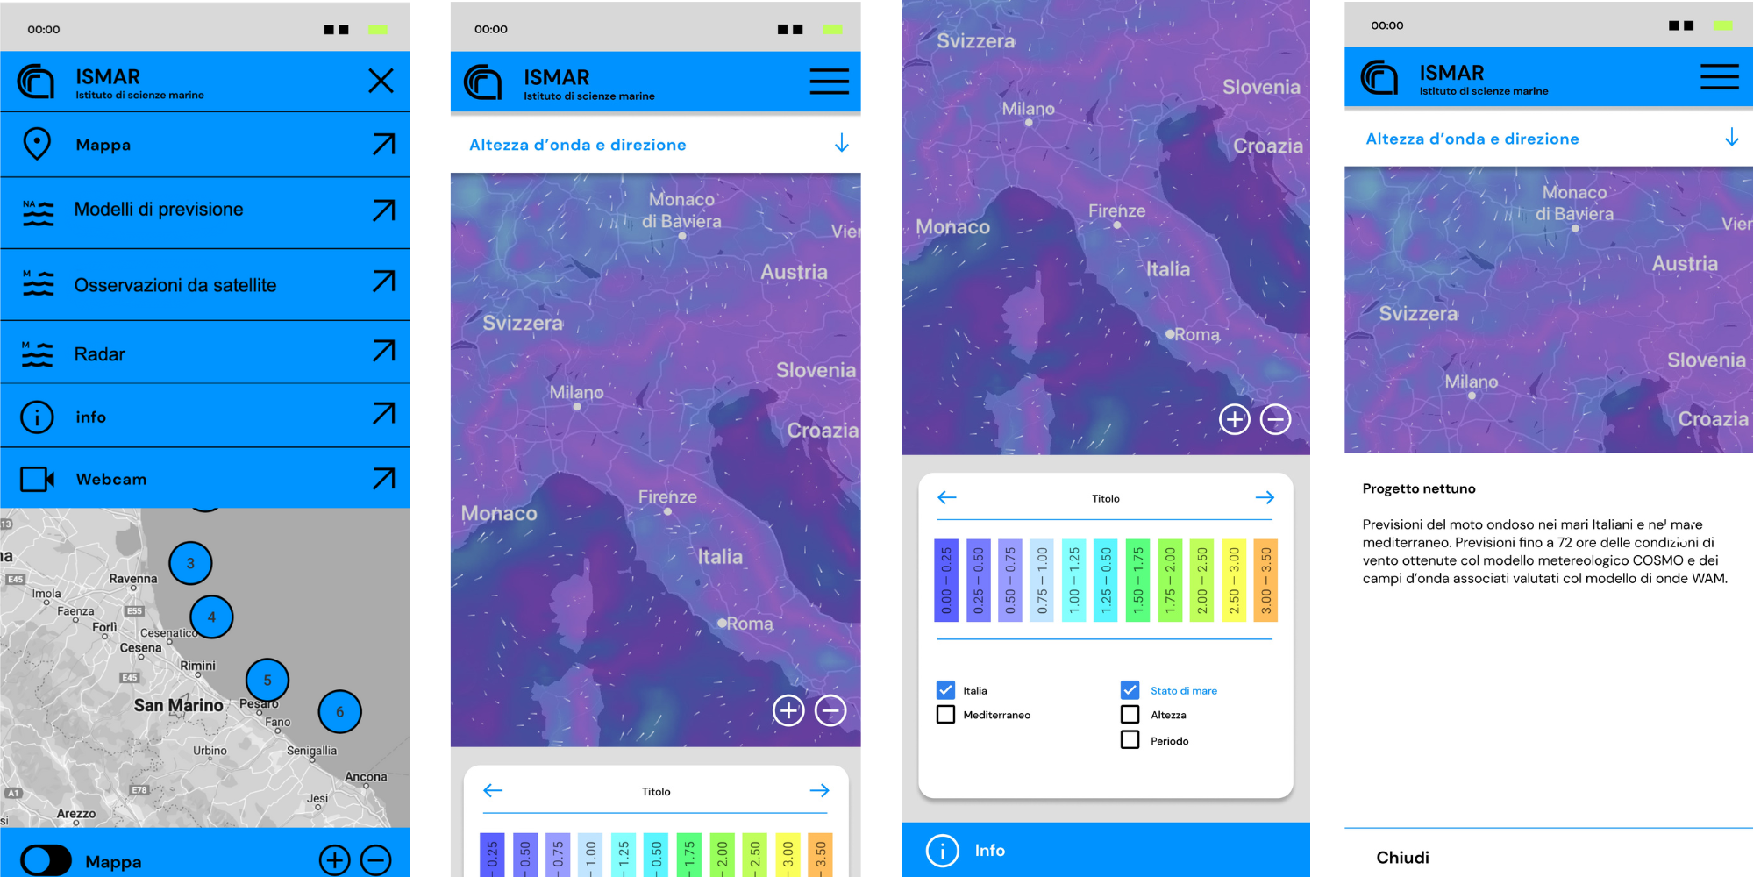
\includegraphics[width=\textwidth]{images/app_ismar_data_menu_nettuno.pdf}
\captionsetup{font=small, hypcap=false}
\captionof{figure}{Schermate menu principale e previsioni onde e vento Nettuno\protect\footnote{Fonte: mockup grafico.}.}
\label{fig:app_menu_henetus}
\end{minipage}
\vspace{0.25cm}
\end{figure}

Per quanto riguarda le webcam, osservabili in \autoref{fig:app_menu_webcam}, esse sono un esempio di funzionalità desiderata ma non implementata. Il motivo è semplice, inizialmente il cliente la considerava una funzionalità fondamentale ma, con il passare del tempo, si è reso conto che ci sono altre priorità. Quindi le webcam restano ma solo come funzionalità da aggiungere nelle versioni future dell'applicazione. 

\begin{figure}[!ht]
\noindent\begin{minipage}{\textwidth}
\vspace{1cm}
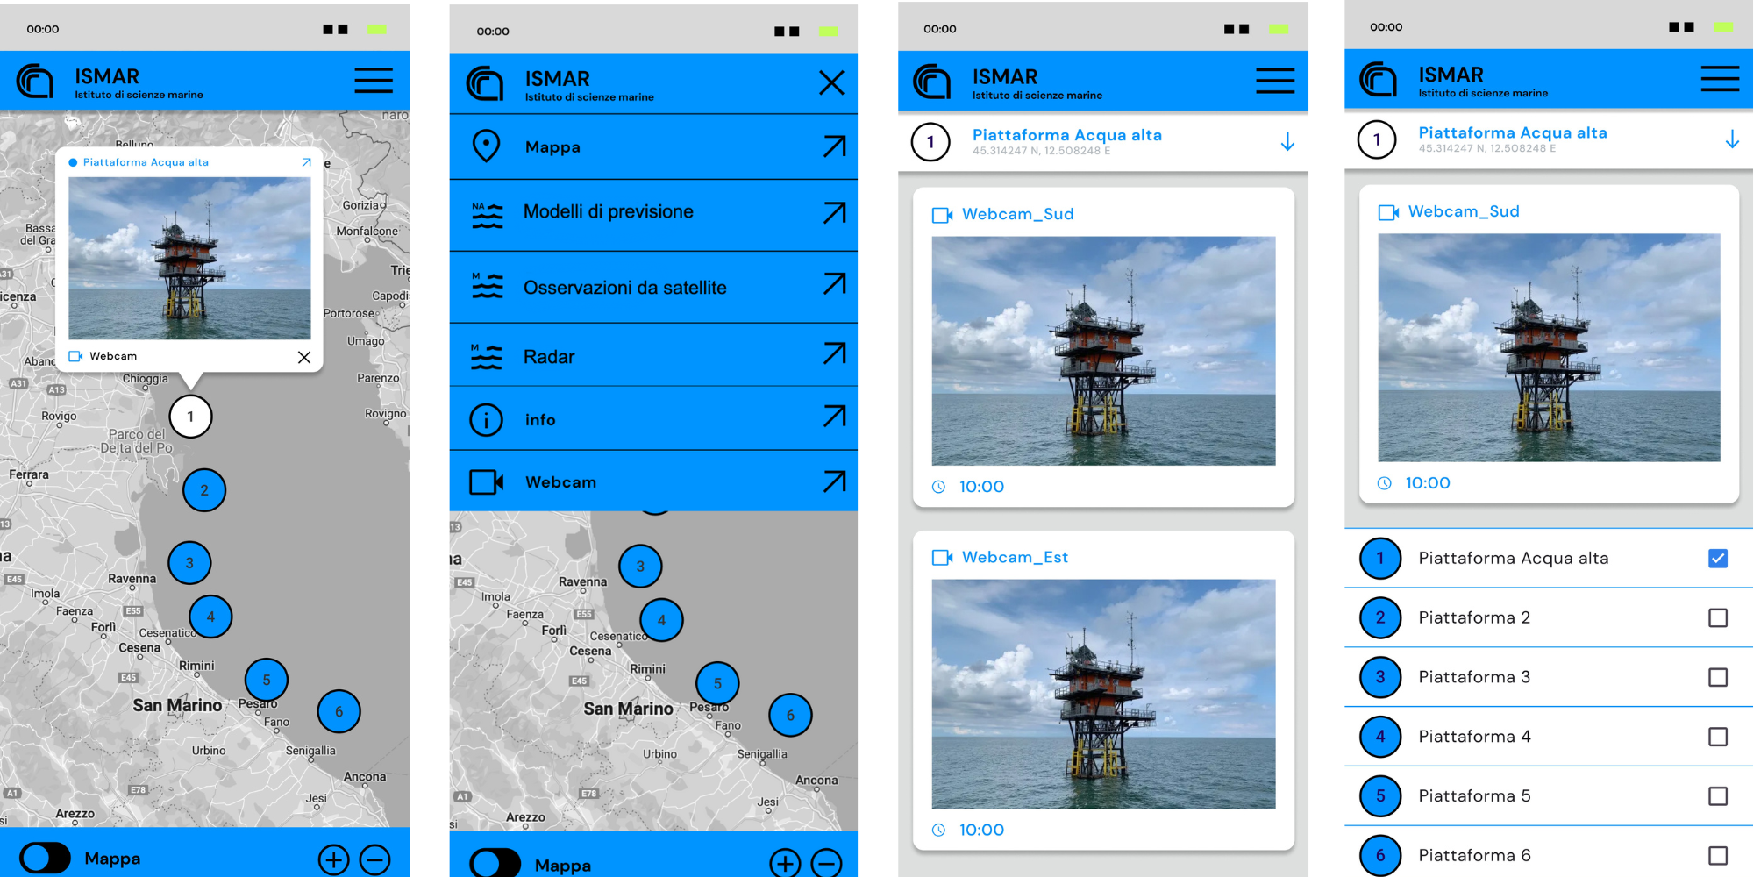
\includegraphics[width=\textwidth]{images/app_ismar_data_webcam.pdf}
\captionsetup{font=small, hypcap=false}
\captionof{figure}{Schermate webcam.\protect\footnote{Fonte: mockup grafico.}.}
\label{fig:app_menu_webcam}
\end{minipage}
\vspace{0.25cm}
\end{figure}

%\paragraph{Back-end.}
Il \textbf{back-end} è il lato che si occupa di reperire i dati, elaborarli e passarli al front-end. Esso fornisce funzionalità di importazione dei dati provenienti dalle diverse sorgenti (stazioni, radar e satelliti) nel modo più generale possibile, favorendo il riuso del codice. I dati importati vengono poi elaborati e semplificati in modo da essere passati al front-end senza che esso abbia necessità di compiere operazioni complicate, le quali diminuiscono la velocità dell'applicazione. Devono essere poi implementati meccanismi per l'aggiornamento dei dati, mantenendoli per un determinato periodo di tempo e di conseguenza eliminando le informazioni meno recenti. Inoltre dovrà essere creato un database per il salvataggio dei dati provenienti dalle varie sorgenti e per altre informazioni utili al funzionamento dell'applicazione. Quindi dovranno essere esposte delle API che si occupano di reperire informazioni dal database locale e di passarle al front-end per la visualizzazione.\par
%Sicuramente quanto detto fin'ora non risulta chiaro, sono presenti termini tecnici e motivazioni che necessitano di un'analisi approfondita. Nelle successive sezioni tutto questo acquisirà un senso, per ora basti sapere che questa è una breve lista di funzionalità ritenute importanti per lo sviluppo del back-end.

L'applicazione, una volta conclusa e approvata dal cliente, dovrà essere disponibile a tutti gli utenti. Questo significa che potrà essere scaricata dai principali marketplace -- \textit{negozi online} -- esistenti: \textbf{Google Play Store} e \textbf{Apple Store}. Questo rientra nelle funzionalità perché, nello sviluppo, è necessario avere in mente dove si vuole arrivare. Quindi l'obbiettivo è creare un'applicazione mobile disponibile per tutti gli utenti, a prescindere dal loro sistema operativo.\par

\end{document}
